\documentclass{article}
\usepackage{xcolor}
\usepackage{titleps}
\usepackage[letterpaper, margin=0.95in]{geometry}
\usepackage{url}
\usepackage{amsmath}
\usepackage{amssymb}
\usepackage{wrapfig}
\usepackage{float}
\usepackage{mathtools}
\usepackage{enumitem}
\usepackage{tabu}
\usepackage{parskip}
\usepackage{natbib}
\usepackage{amsmath}
\usepackage{bbm}
\usepackage{comment}
\usepackage{listings}
\usepackage{graphicx}

\newcommand{\xb}{\mathbf{x}}
\newcommand{\yb}{\mathbf{y}}
\newcommand{\wb}{\mathbf{w}}
\newcommand{\Xb}{\mathbf{X}}
\newcommand{\Yb}{\mathbf{Y}}
\newcommand{\tr}{^T}
\newcommand{\hb}{\mathbf{h}}
\newcommand{\Hb}{\mathbf{H}}
\def\D{\mathcal{D}}
\def\S{\mathcal{S}}
\def\A{\mathcal{A}}
\def\s{\mathbf{s}}
\def\a{\mathbf{a}}
\def\E{\mathbb{E}}
\def\R{\mathcal{R}}
\def\RR{\mathbb{R}}
\def\pib{\pi_{\beta}}


\usepackage{hyperref}
\hypersetup{
    colorlinks=true,
    linkcolor=blue,
    filecolor=blue,      
    urlcolor=blue,
    pdftitle={285 HW 5},
    citecolor=blue,
}

\DeclareFontShape{OT1}{cmtt}{bx}{n}{<5><6><7><8><9><10><10.95><12><14.4><17.28><20.74><24.88>cmttb10}{}


\usepackage{forest}


\usepackage{todonotes}
\usepackage{forest}
\definecolor{light-yellow}{HTML}{FFE5CC}

\newpagestyle{ruled}
{\sethead{Berkeley CS 285}{Deep Reinforcement Learning, Decision Making, and Control}{Fall 2023}\headrule
  \setfoot{}{}{}}
\pagestyle{ruled}

\renewcommand\makeheadrule{\color{black}\rule[-.75\baselineskip]{\linewidth}{0.4pt}}
\renewcommand*\footnoterule{}

\begin{document}
\lstset{basicstyle = \ttfamily,columns=fullflexible,
backgroundcolor = \color{light-yellow}
}

\begin{centering}
    {\Large Assignment 5: Exploration Strategies and Offline Reinforcement Learning} \\
    \vspace{.25cm}
    \textbf{Due Tuesday, November 21, 11:59 pm} \\
\end{centering}

\section{Analysis}
\label{sec:analysis}
\def\H{\mathcal{H}}

In this section, we will analyze how reward bonuses can be used to manage distribution shift in offline RL. We consider an MDP $M=(\S,\A,r,p)$ with offline data $\D$ collected by a policy $\pib$. We denote by $p_\pi$ the distribution over states induced by $\pi$.


As a motivating example, consider the soft actor-critic (SAC) algorithm discussed in HW 3. When updating, SAC adds an adjustment of $b(\s,\a)=-\log \pi(\a\mid\s)$ to the target values $\E_{\pi(\a\mid\s)}[Q(\s,\a)+b(\s,\a)]$ to enforce a maximum entropy regularizer on the policy. Alternatively, we could impose a similar form of entropy regularization by adding the bonus directly to the reward. In expectation, we would optimize \begin{align*}
  \E_{s,a\sim p_\pi} [r(\s,\a)+\lambda b(\s,\a)] 
  &= \tfrac1H J(\pi)-\lambda\,\E_{s\sim p_\pi}\E_{\pi(\a\mid\s)}\log \pi(\a\mid\s) \\
  &= \tfrac1H J(\pi)+\lambda\,\E_{s\sim p_\pi}\H[\pi(\a\mid\s)].
\end{align*}
Thus, entropy regularization can also be implemented by adding the bonus $b(\s,\a)$ to rewards. In the following parts, you will show how a similar reward bonus can be used to constrain distribution shift in offline RL.


We wish to learn a $Q$ function and policy $\pi$ from the offline data $\D$ under some constraint $D(\pi,\pib)\leq\varepsilon$ with the following update:\begin{align}
   Q(\s,\a) &\gets {r}(\s,\a)+\E_{\a' \sim \pi}\left[Q\left(\s',\a'\right)\right] \label{eq:q_update}\\
   \quad &\text{where}\quad \pi=\arg\max_\pi \E_{\s,\a\sim p_\pi} [Q(\s,\a)]\ \text{ s.t. } D(\pi,\pib)\leq\varepsilon. \label{eq:policy_update}
\end{align}
Directly enforcing the constraint in \eqref{eq:policy_update} is challenging with the environment rewards $r(\s,\a)$, so we will implicitly enforce the constraint with a Lagrangian, modifying the reward to $\bar r(\s,\a)=r(\s,\a)+\lambda b(\s,\a)$ in \eqref{eq:q_update}. The overall optimization then becomes:
\begin{align}
   Q(\s,\a) &\gets \bar{r}(\s,\a)+\E_{\a' \sim \pi}\left[Q\left(\s',\a'\right)\right] \\
   \quad &\text{where}\quad \pi=\arg\max_\pi \E_{\s,\a\sim p_\pi} [Q(\s,\a)].
\end{align}
You may assume that $\lambda>0$ is selected appropriately to enforce the constraint as follows: $$\left(\arg\max_\pi \E_{\s,\a\sim p_\pi} [Q(\s,\a)]-\lambda D(\pi,\pi_\beta)\right)=\left(\arg\max_\pi \E_{\s,\a\sim p_\pi} [Q(\s,\a)]\ \text{ s.t. } D(\pi,\pib)\leq\varepsilon\right).$$
You may also assume access to the distributions $\pi(\a\mid\s)$ and $\pib(\a\mid\s)$ in your answers.

\begin{enumerate}

	\item\label{q:kl} Suppose we wish to learn $\pi$ under a KL-divergence constraint, i.e., 
	\begin{align*}
		D(\pi,\pib)=\E_{\s\sim p_\pi}D_{KL}[\pi(\a\mid\s)\|\pib(\a\mid\s)].
	\end{align*}
	How can we enforce this constraint by adding a bonus $b(\s,\a)$ to the reward $\bar r(\s,\a)=r(\s,\a)+\lambda b(\s,\a)$? Write your answer as an expression for $b(\s,\a)$.
	
	\item The $f$-divergence is a generalization of the KL-divergence that can be defined for distributions $P$ and $Q$ by $$D_f[P\|Q]=\int Q(x)f\left(P(x) \over Q(x)\right)\mathrm dx$$ where $f$ is a convex function with zero at $1$. We can state an $f$-divergence policy constraint as 
	\begin{align*}
	    D(\pi,\pib)&=\E_{\s\sim p_\pi}D_{f}[\pi(\a\mid\s)\|\pib(\a\mid\s)]\\
	    &= \E_{\s\sim p_\pi}\E_{\pib(\a\mid\s)}f\left(\pi(\a\mid\s)\over\pib(\a\mid\s)\right).
   	\end{align*}
   	The $f$-divergence constraint allows us to specify many alternative constraints on the divergence between $\pi$ and $\pib$. For example, by taking $f(x)=\frac12|x-1|$, the $f$-divergence becomes equivalent to total variation distance (TVD), and by taking $f(x)=-(x+1)\log\left(x+1\over2\right)+x\log x$ it reduces to the Jensen-Shannon divergence (JSD). When $f(x)=x\log x$ we recover the standard KL divergence.
   	
   	How can you extend your answer from part (\ref{q:kl}) to account for an arbitrary $f$-divergence? Your answer should be a more general alternate expression for $b(\s,\a)$ in terms of $f$.
	\item Suppose $M$ has a finite horizon $H$ and we want to constrain divergence in the distribution of \emph{trajectories of states} under $\pi$ and $\pib$. We can express the KL divergence between the (state) trajectory distributions for $\tau=(\s_1,\s_2,\ldots,\s_H)$ as follows:
	\begin{align*}
	    D(\pi,\pib)&=D_{KL}[p_{\pi}(\tau)\|p_{\pib}(\tau)].
   	\end{align*} 
   	What expression for $b(\s,\a)$ enforces this constraint? You may assume access to the dynamics $p(\s'\mid\s,\a)$. [\emph{Hint: marginalize over actions to get a bonus $b(\s,\a,\s')$ that depends on $\s'$. How can this be converted to a bonus $b(\s,\a)$ that can be used with $r(\s,\a)$?}]

\end{enumerate}

\section{Coding}
\label{sec:coding}
This section requires you to implement and evaluate a pipeline for exploration and offline learning. You will first implement an exploration method called random network distillation (RND) and collect data using this exploration procedure, then perform offline training on the data collected via RND using conservative Q-learning (CQL), Advantage Weighted Actor Critic (AWAC), and Implicit Q-Learning (IQL). 
This assignment will be easier to run on a CPU as we will be using gridworld domains of varying difficulties to train our agents. 

The questions will require you to perform multiple runs of offline RL training, which can take quite a long time as we ask you to analyze the empirical significance of specific hyperparameters and thus sweep over them. Furthermore, depending on your implementation, you may find it necessary to tweak some of the parameters, such as learning rates or exploration schedules, which can also be very time consuming. We would $\textbf{highly}$ recommend starting early on the coding to allocate enough time to finish the assignment effectively.

\subsection{File overview}
The starter code for this assignment can be found at

\begin{centering}
\url{https://github.com/berkeleydeeprlcourse/homework_fall2023/tree/master/hw5} \\
\end{centering}
\vspace{.35cm}

All files needed to run your code are in the \texttt{hw5} folder. 
You will be writing new code in the following files (all in the \texttt{hw5/cs285/agents} folder):
\begin{itemize}
\item \texttt{random\_agent.py}
\item \texttt{rnd\_agent.py}
\item \texttt{dqn\_agent.py}
\item \texttt{cql\_agent.py}
\item \texttt{awac\_agent.py}
\item \texttt{iql\_agent.py}
\end{itemize}


\begin{figure}[h]
    \centering
    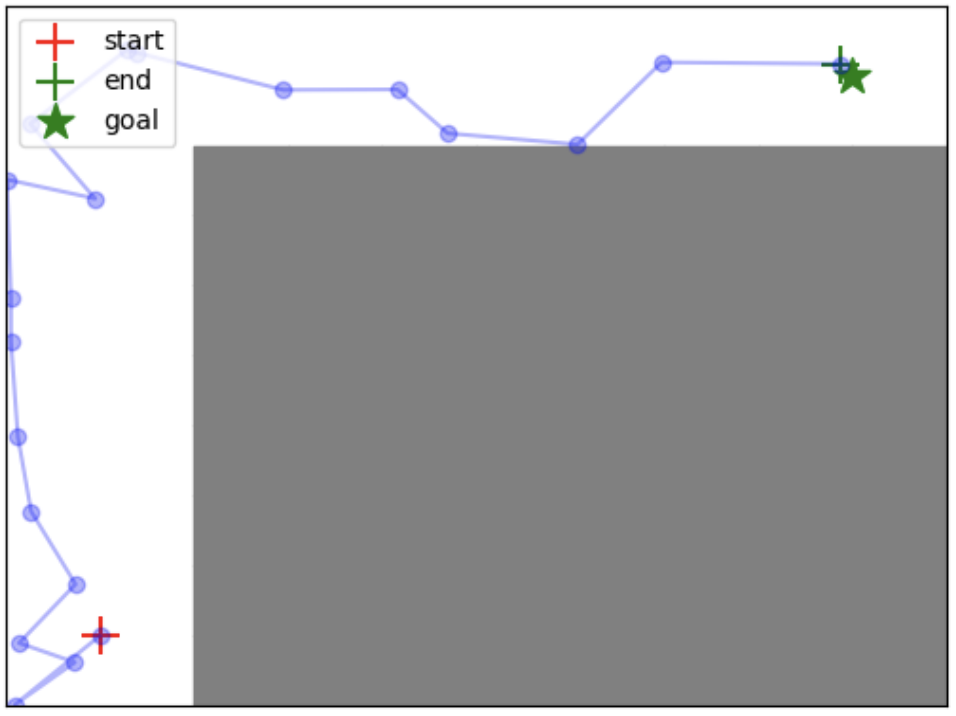
\includegraphics[width=0.32\textwidth]{easy.png}~
    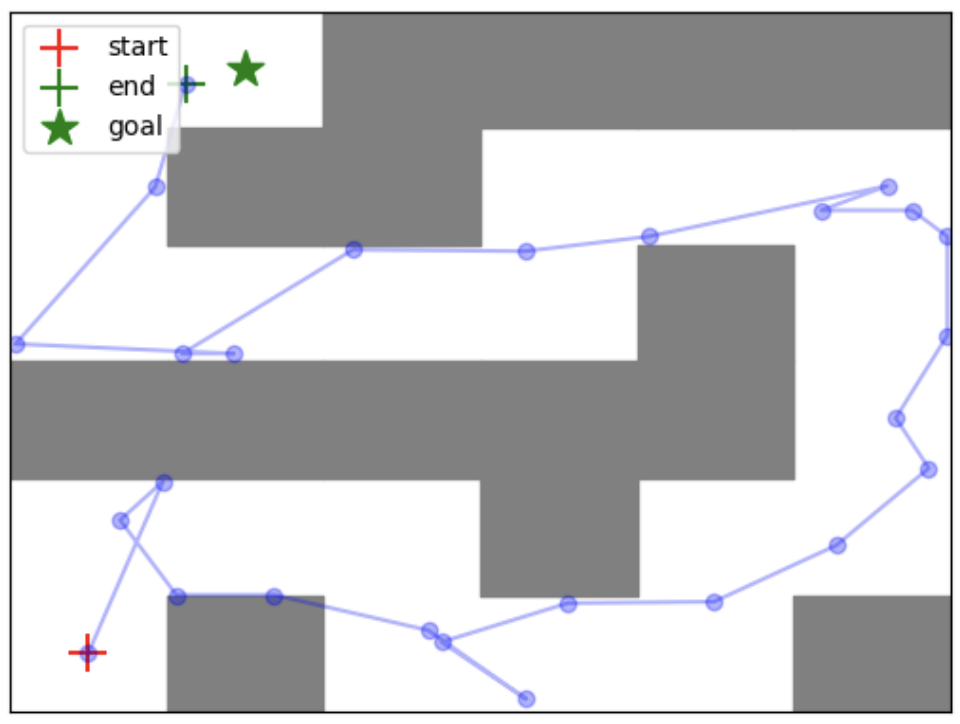
\includegraphics[width=0.32\textwidth]{medium.png}~
    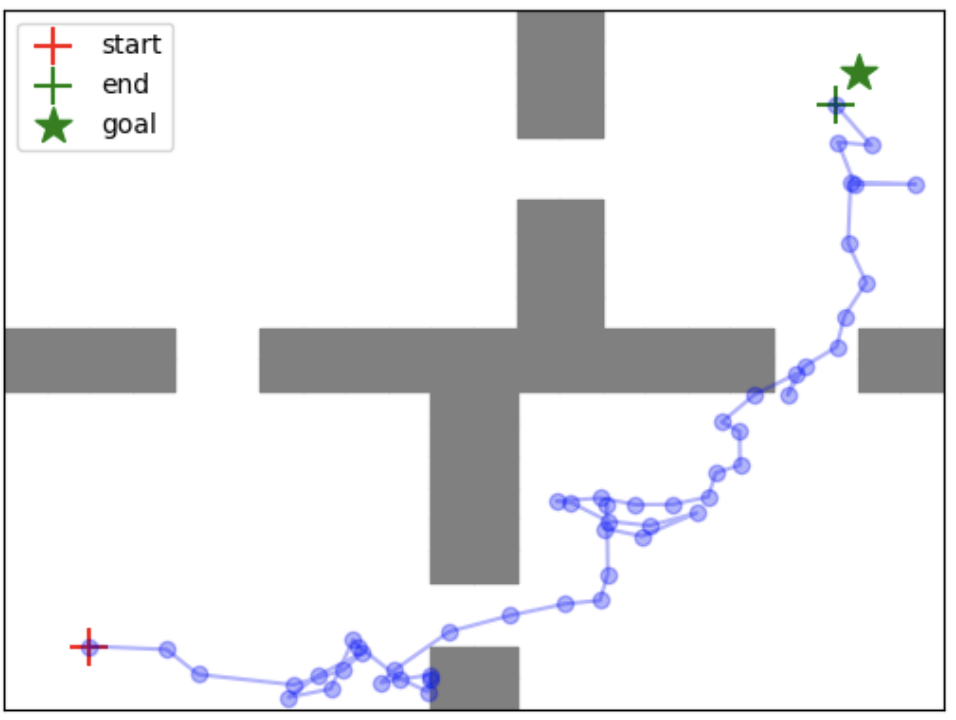
\includegraphics[width=0.32\textwidth]{hard.png}
    \vspace{-10pt}
    \caption{Figures depicting the \texttt{easy} (left), \texttt{medium} (middle) and \texttt{hard} (right) environments.}
    \vspace{-10pt}
\end{figure}
\subsection{Environments}
Unlike previous assignments, we will consider some stochastic dynamics, discrete-action gridworld environments in this assignment. The three gridworld environments you will need for the graded part of this assignment are of varying difficulty: \texttt{easy}, \texttt{medium} and \texttt{hard}. A picture of these environments is shown below. The easy environment requires following two hallways with a right turn in the middle. The medium environment is a maze requiring multiple turns. The hard environment is a four-rooms task which requires navigating between multiple rooms through narrow passages to reach the goal location. We also provide a very hard environment for the bonus (optional) part of this assignment.

\subsection{Random Network Distillation (RND) Algorithm}
A common way of doing exploration is to visit states with a large prediction error of some quantity, for instance, the TD error or even random functions. The RND algorithm, as covered in Lecture 13, aims at encouraging exploration by asking the exploration policy to more frequently undertake transitions where the prediction error of a random neural network function is high. Formally, let ${f}_\theta^*(s')$ be a randomly chosen vector-valued function represented by a neural network. RND trains another neural network, $\hat{f}_\phi(s')$ to match the predictions of $f^*_\theta(s')$ under the distribution of datapoints in the buffer, as shown below:
\begin{equation}
    \phi^* = \arg \min_\phi~ \mathbb{E}_{s, a, s' \sim \mathcal{D}} \left[\underbrace{||\hat{f}_\phi(s') - f^*_\theta(s')||}_{\mathcal{E}_\phi(s')} \right].
\end{equation}
If a transition $(s, a, s')$ is in the distribution of the data buffer, the prediction error $\mathcal{E}_\phi(s')$ is expected to be small. On the other hand, for all unseen state-action tuples it is expected to be large. To utilize this prediction error as a reward bonus for exploration, RND trains two critics -- an \emph{exploitation critic}, $Q_R(s, a)$, and an \emph{exploration critic}, $Q_\mathcal{E}(s, a)$, where the exploitation critic estimates the return of the policy under the actual reward function and the exploration critic estimates the return of the policy under the reward bonus. In practice, we normalize error before passing it into the exploration critic, as this value can vary widely in magnitude across states leading to poor optimization dynamics.

In this problem, we represent the random functions utilized by RND, $f^*_\theta(s')$ and $\hat{f}_\phi(s')$ via random neural networks. To prevent the neural networks from having zero prediction error right from the beginning, we initialize the target $f^*_\theta$ using an alternative initialization scheme in \verb+agents/rnd_agent.py+. 

\subsection{Conservative Q-Learning (CQL) Algorithm}
For the first portion of the offline RL part of this assignment, we will implement the conservative Q-learning (CQL) algorithm. The goal of CQL is to preventing overestimation of the policy value. In order to do that, a conservative, lower-bound Q-function is learned by additionally minimizing Q-values alongside a standard Bellman error objective. This is done by augmenting the Q-function training with a regularizer that minimizes the soft-maximum of the Q-values $\log \left( \sum_{a} \exp(Q(s, a)) \right)$ and maximizes the Q-value on the state-action pair seen in the dataset, $Q(s, a)$. The overall CQL objective is given by the standard TD error objective augmented with the CQL regularizer weighted by $\alpha$: $\alpha \left[\frac{1}{N}\sum_{i=1}^N \left(\log\left(\sum_{a} \exp(Q(s_i, a))\right) - Q(s_i, a_i) \right) \right]$. You will tweak this value of $\alpha$ in later questions in this assignment.  

\subsection{Advantage Weighted Actor Critic (AWAC) Algorithm}
For the second portion of the offline RL part of this assignment, we will implement the AWAC algorithm. This augments the training of the policy by utilizing the following actor update:

\begin{equation}
    \theta \leftarrow \arg \max_\theta~ \mathbb{E}_{s, a \sim \mathcal{B}} \left[\log \pi_{\theta}(a|s) \exp(\frac{1}{\lambda} \mathcal{A}^{\pi_{k}}(s,a)) \right].
\end{equation}

This update is similar to weighted behavior cloning (which it resolves to if the Q function is degenerate). But with a well-formed Q estimate, we weight the policy towards selecting actions that are high under our learnt q function. In the update above, the agent regresses onto high-advantage actions with a large weight, while almost ignoring low-advantage actions. This actor update amounts to weighted maximum likelihood (i.e., supervised learning), where the targets are obtained by re-weighting the state-action pairs observed in the current dataset
by the predicted advantages from the learned critic, without
explicitly learning any parametric behavior model, simply
sampling (s, a) from the replay buffer $\beta$. 

The Q function is learnt with a Temporal Difference (TD) Loss. The objective can be found below.
\begin{equation}
    \mathbb{E}_{D}[(Q(s,a) - r(s,a) + \gamma\mathbb{E}_{a' \sim \pi}[Q_{\phi_{k-1}}(s',a')])^2]
\end{equation}

Note that next actions $a'$ are sampled from the learned policy $\pi$, meaning that OOD actions will not be sampled if $\pi$ does a good job of fitting the (weighted) behavior policy.

\subsection{Implicit Q-Learning (IQL) Algorithm}

For the second portion of the offline RL part of this assignment, we will implement the IQL algorithm. IQL decouples the problem of learning the critic from the policy learning by using an \textit{implicit} Bellman backup rather than explicitly considering the backup under a particular policy. It does this by learning an \textit{expectile} of $Q$, which is a statistic similar to a quantile. This is a ``soft'' version of the \textit{maximum} value attained by a distribution. For a random variable $X$, the expectile $m_\tau(X)$ is given as to minimize the following:
\[\arg \min_{m_\tau} \mathbb{E}_{x \sim X}[L_2(x - m_\tau)], L_2^\tau(\mu) = |\tau - \mathbbm{1}\{ \mu \le 0 \} |\mu^2\]
This backup will act optimistically with respect to actions taken in the dataset. To avoid being optimistic to \textit{state} transitions, we need to learn a separate value function $V(s)$ that performs the optimism, then regress $Q(s, a) \gets r + \gamma V(s')$ with a regular MSE loss. All together:
\begin{equation}
    L_V(\phi) =  \mathbb{E}_{(s,a) \sim D}[L_2^\tau(Q_\theta(s,a) - V_\phi(s))]
\end{equation}

\begin{equation}
    L_Q(\theta) =  \mathbb{E}_{(s,a,s') \sim D}[(r(s,a) + \gamma V_\phi(s') - Q_\theta(s,a))^2]
\end{equation}

Note that the critic learning process has two nice properties:
\begin{enumerate}
    \item It never queries out-of-distribution actions (e.g. actions $a'$ from an arbitrary policy), which completely avoids the OOD overestimation issue.
    \item It can be conducted without an actor update, so if you want you can first train a critic and then only train the actor at the end.
\end{enumerate}

The actor update is decoupled from the critic update (hence \textit{implicit} $Q$-learning), and is learned with the same objective as AWAC:
\begin{equation}
    L_\pi(\psi) = -\mathbb{E}_{s, a \sim \mathcal{B}} \left[\log \pi_{\psi}(a|s) \exp(\frac{1}{\lambda} \mathcal{A}^{\pi_{k}}(s,a)) \right].
\end{equation}

\subsection{Relevant Literature}
For more details about the algorithmic implementation, feel free to refer to the following papers: \href{https://arxiv.org/abs/2006.04779}{Conservative Q-Learning for Offline Reinforcement Learning (CQL)}, \href{https://arxiv.org/abs/2006.09359}{Accelerating Online Reinforcement Learning with Offline Datasets (AWAC)}, \href{https://arxiv.org/abs/1810.12894}{Offline Reinforcement Learning with Implicit Q-Learning (IQL)}, and \href{https://arxiv.org/abs/2110.06169}{Exploration by Random Network Distillation (RND)}.

\subsection{Implementation}
The first part in this assignment is to implement a working version of Random Network Distillation. The default code will run the \texttt{easy} environment with reasonable hyperparameter settings. Look for the \texttt{\# TODO(student)} markers in the files listed above for detailed implementation instructions.
\subsection{Evaluation}

Once you have a working implementation of RND, CQL, AWAC, and IQL, you should prepare a report. The report should consist of one figure for each question below (each part has multiple questions). You should turn in the report as one PDF and a zip file with your code. If your code requires special instructions or dependencies to run, please include these in a file called \verb+README+ inside the zip file.

\section{Exploration}
In RL, our agent needs to see high-reward transitions at some point during training to understand that they exist. Your previous assignments (PG, DQN, SAC) have just used random exploration, possibly with some state-dependent noise (like in SAC). Here, you'll instead implement a policy that explicitly maximizes state coverage to explore the entire space.

Later, we'll use data collected from these exploration policies with several different offline RL algorithms.

\subsection{Running a random policy}
Just to get a sense for the three environments, implement \verb+get_action+ for the \verb+RandomAgent+ in \verb+random_agent.py+. Run the random policy to generate random exploration in each of the three environments:
\begin{lstlisting}[language=bash]
python cs285/scripts/run_hw5_explore.py \
    -cfg experiments/exploration/pointmass_easy_random.yaml
    --dataset_dir datasets/
python cs285/scripts/run_hw5_explore.py \
    -cfg experiments/exploration/pointmass_medium_random.yaml \
    --dataset_dir datasets/
python cs285/scripts/run_hw5_explore.py \
    -cfg experiments/exploration/pointmass_hard_random.yaml \
    --dataset_dir datasets/
\end{lstlisting}
These scripts will save visualizations of the final dataset in the \verb+exploration+ directory, as well as intermediate results in the Tensorboard logs. Include the final dataset visualization in your report.

\subsection{Random Network Distillation}
\textbf{What you will implement}: the RND algorithm for exploration. You will need to change \verb+cs285/agents/rnd_agent.py+. In addition, you should also thoroughly read through the training scheme in \verb+run_hw5_explore.py+. It's very similar to the DQN training scheme you implemented in HW3.

Implement the RND algorithm and use the argmax policy with respect to the exploration critic to generate state-action tuples to populate the replay buffer for the algorithm. In the code, this happens before the number of iterations crosses \verb+num_exploration_steps+, which is set to 10k by default. You need to collect data using the \verb+ArgmaxPolicy+ policy which chooses to perform actions that maximize the exploration critic value.

The experiment logs contain visualizations of RND error computed at each point in the environment as well as a scatter plot of visited states. As exploration progresses, a working RND algorithm should accumulate low error in all reachable states and high error in unreachable states (e.g. walls).

First, make sure your RND implementation works in the easy environment. Then, run it in all three environments:
\begin{lstlisting}[language=bash]
python cs285/scripts/run_hw5_explore.py \
    -cfg experiments/exploration/pointmass_easy_rnd.yaml
    --dataset_dir datasets/
python cs285/scripts/run_hw5_explore.py \
    -cfg experiments/exploration/pointmass_medium_rnd.yaml \
    --dataset_dir datasets/
python cs285/scripts/run_hw5_explore.py \
    -cfg experiments/exploration/pointmass_hard_rnd.yaml \
    --dataset_dir datasets/
\end{lstlisting}

Again, include the visualizations in your final report. \textbf{These visualizations, particularly the RND error map, will be very helpful for debugging!}

\section{Offline RL}

\subsection{CQL}
Now that we have implemented RND for collecting exploration data that is (likely) useful for performing exploitation, we will perform offline RL on this dataset and see how close the resulting policy is to the optimal policy. To begin, you will implement the conservative Q-learning algorithm in this \verb+cs285/agents/cql_agent.py+.

Then, run both a standard DQN agent and your new CQL agent in the offline setting with the datasets you collected earlier.

\begin{lstlisting}[language=bash]
python ./cs285/scripts/run_hw5_offline.py \
    -cfg experiments/offline/pointmass_easy_cql.yaml \
    --dataset_dir datasets
python ./cs285/scripts/run_hw5_offline.py \
    -cfg experiments/offline/pointmass_medium_dqn.yaml \
    --dataset_dir datasets

python ./cs285/scripts/run_hw5_offline.py \
    -cfg experiments/offline/pointmass_easy_cql.yaml \
    --dataset_dir datasets
python ./cs285/scripts/run_hw5_offline.py \
    -cfg experiments/offline/pointmass_medium_dqn.yaml \
    --dataset_dir datasets
\end{lstlisting}

On the Medium environment, create several experiment variations in which the value of the $\alpha$ parameter is varied, from $\alpha=0$ (equivalent to DQN) to $\alpha=10$. Show both resulting $Q$-values and evaluation performances in a plot. In the caption, describe how the $\alpha$ parameter affects training and performance in offline RL.

\subsection{Policy Constraint Methods: IQL and AWAC}
While CQL learns an actor via a modification to actor-critic algorithms like DQN that regularizes actions towards those found in the dataset by decreasing OOD $Q$-values, AWAC learns an in-distribution policy directly by performing weighted behavior cloning on the dataset.

Implement AWAC in \verb+cs285/agents/awac_agent.py+, and IQL in \verb+cs285/agents/iql_agent.py+. Compare them using the IQL and AWAC configuration files in the \verb+experiments+ directory. Report evaluation curves for both approaches.

\subsection{Data ablations}
Finally, compare the performance of offline RL under several different sizes of dataset. Run RND with \verb+total_steps+ 1000, 5000, 10000, and 20000 on either the Medium or Hard environment, creating a new dataset for each variation (you will need to make several .yaml config files for this). Then, train a CQL agent on each dataset and report its performance as well as evaluation curves.

\section{Online Fine-Tuning}
So far we only support training an algorithm purely offline, using data collected in a previous run. In \verb+run_hw5_finetune.py+, implement online fine-tuning by first loading an offline dataset and taking a fixed number of training steps with an offline RL algorithm of your choice (IQL, CQL, or AWAC) and then switching to online learning while keeping all of the data in the dataset to initialize your replay buffer.

Report results as evaluation returns, clearly indicating the point at which online fine-tuning begins. An example configuration is provided for you in \verb+experiments/finetune/pointmass_hard_cql_finetune.yaml+.

With online fine-tuning, your policy should be able to (stably) reach high reward (at least -20) on \verb+PointmassHard-v0+.

\section{Submitting the code and experiment runs}
In order to turn in your code and experiment logs, create a folder that contains the following: 
\begin{itemize}
    \item A folder named \texttt{data} with all the experiment runs from this assignment.
    \textbf{Do not change the names originally assigned to the folders, as specified by  \texttt{exp\_name} in the instructions. Video logging is not utilized in this assignment, as visualizations are provided through plots, which are outputted during training.}
    \item The \texttt{cs285} folder with all the \texttt{.py} files, with the same names and directory structure as the original homework repository (excluding the \texttt{data} folder). Also include any special instructions we need to run in order to produce each of your figures or tables (e.g. ``run python myassignment.py -sec2q1'' to generate the result for Section 2 Question 1) in the form of a README file.
\end{itemize}

If you are a Mac user, \textbf{do not use the default ``Compress'' option to create the zip}. It creates artifacts that the autograder does not like. You may use \texttt{zip -vr submit.zip submit -x "*.DS\_Store"} from your terminal.

Turn in your assignment on Gradescope. Upload the zip file with your code and log files to \textbf{HW5 Code}, and upload the PDF of your report to \textbf{HW5}.

As an example, the unzipped version of your submission should result in the following file structure. \textbf{Make sure that the submit.zip file is below 15MB and that they include the prefix \texttt{q1\_}, \texttt{q2\_}, \texttt{q3\_}, etc.}

\begin{forest}
  for tree={
    font=\ttfamily,
    grow'=0,
    child anchor=west,
    parent anchor=south,
    anchor=west,
    calign=first,
    edge path={
      \noexpand\path [draw, \forestoption{edge}]
      (!u.south west) +(7.5pt,0) |- node[fill,inner sep=1.25pt] {} (.child anchor)\forestoption{edge label};
    },
    before typesetting nodes={
      if n=1
        {insert before={[,phantom]}}
        {}
    },
    fit=band,
    before computing xy={l=15pt},
  }
[submit.zip
  [data
      [q1...
        [events.out.tfevents.1567529456.e3a096ac8ff4]
      ]
      [...]
  ]
  [cs285
    [...]
  ]
    [...]
]
\end{forest}

\end{document}